% This is LLNCSDE2.TEX, a variation of LLNCS.DEM
% (the demonstration file of
% the LaTeX macro package from Springer-Verlag
% for Lecture Notes in Computer Science,
% version 2.2 for LaTeX2e),
% which can be used by volume editors for the preparation
% of the front matter pages and the author index
%
% Last changes: 04.08.1999, Antje Endemann (endemann@springer.de)
%
%%%%%%%%%%%%%%%%%%%%%%%%%%%%%%%%%%%%%%%%%%%%%%%%%%%%%%%%%%%%%%%%%%%%%
% In order to generate an Author Index do the following:
% After TeXing this document start the program MakeIndex by typing
% MAKEINDX -S SPRMINDX.STY <filename>
% (generates an IND file for the Author Index)
% into the DOS command line.
% (At other systems you may have to use the command MAKEINDEX.)
% Now TeX this file once again, then you will get an Author Index.
% TeX this file once more, then the TOC will be complete.
%%%%%%%%%%%%%%%%%%%%%%%%%%%%%%%%%%%%%%%%%%%%%%%%%%%%%%%%%%%%%%%%%%%%%
\documentclass[12 pt,a4paper]{llncs}
%\documentclass{llncs}
%\usepackage{ucs}
\usepackage[utf8]{inputenc}
\usepackage{fancyhdr}
\usepackage[dvips]{graphicx}
\usepackage{graphicx}
\usepackage{fancyhdr,epsfig}
\usepackage{a4wide}
\usepackage{amssymb}
%\parskip 0.5 ex


\begin{document}

\title{Un modelo compresivo para el diseño de procesos en una Aplicación E-Learning }

\author{Alejandro Sartorio}


\index{Ekeland, Ivar}
\index{Temam, Roger}
% use the command \index{<name>} for index entries

\institute{UNR Universidad Nacional de Rosario \and  SecyT}
%\authorinfo{sartorio@fceia.unr.edu.ar}
jfjjfj

jfjhfjh

hfjhj
jfhjjhj



\begin{abstract}
En este trabajo se presenta un modelo comprensivo para el diseño de Transacciones Web que implementan procesos en una Aplicación Web E-Learning. El modelo fue creado en el marco del proyecto Obra Abierta (CONICET-UNR), para el diseño de Requerimentos y Procesos de Ejecución para una Aplicación E-learning. Las Transacciones que se implementan en la Aplicación están formadas con contratos con propiedades context-awareness.

Dicho modelo es una extensión y adaptación del modelo conceptual y de diseño UWAT+ (Ubiquitous Web Application Transaction). Mediante un caso de estudio real, se ejemplificará su aplicación y uso en el proyecto Obra Abierta. 

\end{abstract}

\begin{abstract}
 
hgfhhgfd
hfghdgfhdgfh
hfgdhgfhfghgfd


\end{abstract}

%\small{\textbf{Palabras Claves:} Aplicaciones e-Learning, diseño de transacciones Web, documentación, coordinación de contratos context-aware} 
%

\newpage

\section {INTRODUCCIÓN} \label{intro}

A medida que el avance en la investigación y desarrollo de plataformas e-learning brinden  mejoras e innovaciones de herramientas (videoconferencias, porfolios, wikis, workshops, etc.) y sus respectivos servicios,  crece la cantidad de posibles configuraciones de los espacios e-learning.  Abarcando diferentes tipos de requerimientos pertenecientes a las etapas de diseño, otros durante el desarrollo y otros en tiempo de ejecución. A partir de estos se definen los procesos e-learning (Pe-lrn). Al igual que los procesos de negocios en una aplicación Web convencional (ej., www.ebay.com), los P-elrn están compuesto por transacciones Web \\part{cite}
{transaccion web}. En este contexto, una transacción (o transacción e-learning) es definida como una secuencias de actividades que el usuario ejecuta a través de la aplicación e-learning con el propósito de efectuar una tarea o concretar un objetivo. El conjunto de actividades, sus propiedades y las reglas que goviernan sus ejecuciones dependen del Pe-lrn que la aplicación debe brindar.

Las características tecnológica de un Aplicación Web e-learning (AWe-lrn) son idénticas a las aplicaciones e-learning convencionales (por ejemplo, las utilizadas en el proyecto de e-learning Sakai\footnote{SaKai: Entorno colaborativo y de aprendisaje para enseñar. Es de código abierto y está resuelto con tecnología Java. Url: wwww.sakaiprojet.org}) que proveen:  navegación etre páginas a través de links, ejecución de transacciones e-learning por medio de los servicios de las herramientas y las operaciones de un Pe-lrn. La principal diferencia tecnológica entre un AWe-lrn y una aplicación e-learning convencional es la incorporación de la teoría de coordinación de contratos \cite{fiadeiro,libro5} en la implementación de algunos servicios que las herramientas brindan a los usuarios \cite{libro}.

En base a la incorporación de los contratos en la implementación y diseño de transacciones e-leaning, aumente aún más las posibibles configuraciones de los Pe-lrn. A través de la inclusión de una componente contrato como objeto de primera clase, comienzan a aparecer nuevas propiedas que tienen que ver con el campo de la Ingeniería de Software. Y, a su vez,  fuertemente relacionados al trabajo multidiciplinario entre los actores de un proyecto de contrucción de una AWe-lrn (ej. el proyecto Obra Abierta \footnote{Obra Abierta: Proyecto de I&D (CONICET), que se centra en el desarrollo e implementación de dispositivos hipermediales contex-aware dinámico para investigar y aprender en contextos físicos-virtuales de educación superior. Directora: Patricia San Martín }). Para este fin, es imprescindible contar con un modelo de diseño que ayude en el ciclo de vida del desarrollo y configuración de una aplicación e-learning. Integrando las tareas de los expertos en educación, diseñadores y desarrolladores.

Desde el punto de vista de la ingeniería de software, desatender o resolver incorrectamente la documentación para el diseño de procesos tipo Pe-lrn pueden causar numerosos problemas reflejados en el proceso de configuración  de un AWe-lrn. Estos problemas pueden ser:


\begin{itemize}
	\item Dificultades en la comunicación y entendimiento entre los clientes y diseñadores expertos en educación (primero), y entre los diseñadores y los desarrolladores (después), en el proceso de implementación de un AWe-lrn.

	\item Determinación de las relaciones donde se justifique la inclusión de contratos.
	
	\item Dificultad para visualizar la trazabilidad entre los procesos e-learning y las implementaciones de las transacciones.

\end{itemize}

Este trabajo presenta un diseño compresivo para el modelado de los procesos de educación e investigación (Pe-lrn) en un Aplicación Web E-learning con la inclusión de los contrato con propiedades context-aware \cite{libro}. El modelo está basado en UWAT+ (Distante, 2004), una versión extendida y adaptada de "UWA Transaction Design Model" para el diseño de transacciones en aplicaciones Web. La principales contribuciones de este trabajo son:

\begin{itemize}
 \item El acercameinto de un modelo útil para la represetación de transacciones e-learning en una AWe-lrn; permitiendo una mejor distinción de la ubicación (entre servicio-usuario(s) y servicio-servicio(s)) de la componente contrato dentro del flujo de ejecución.
 \item Ejemplificar, mediante un caso de uso concreto,  el uso del modelo UWATc+.

\end{itemize}

El resto de este trabajo se encuentra organizado de la siguiente manera: Tras esta introducción se presenta una referencia conceptual del los contratos utilizados en el proyecto Obra Abierta (Seccción \ref{contrato}). Luego se continúo con definiciones, formas de documentación y representación de transacciones e-learning, procesos, etc. (sección \ref{documentacion}). Siguiendo, se presenta un modelo conceptual y de diseño sobre la adaptación propuesta para el modelado de Pe-lrn (sección \ref{uwatc}). Aplicado a un caso de uso concreto se describe y aplica el modelo de diseño UWATc+ para cada una de sus etapas. Finalizando con una breve conclusión.


\section{CONTATOS CONTEXT-AWARE PARA TRANACCIONES E-LEARNING} \label{contrato}

En términos generales, la coordinación de contratos es una conexión establecida entre un grupo de objetos (en nuestras consideraciones, un objeto cliente y un determinado servicio serían los participantes), donde reglas, normas y restricciones (RNR) son superpuestas entre los actores participantes, estableciendo con un determinado grado de control las formas de interrelación (o interacción). 
El tipo de interacciones establecidas entre las partes es más satisfactoria que las que se pueden lograr con UML o lenguajes similares (Orientados a Objetos) debido a que éstas contienen un mecanismo de superposición donde se toma como argumento los contextos. Cuando un objeto cliente efectúa una llamada a un objeto suministro, el contrato "intercepta" la llamada y establece una nueva relación teniendo en cuenta el contexto del objeto cliente, el del objeto servidor e información relevante (a la relación) adquirida y representada como contexto del entorno. Como condición necesaria, la implementación de los contratos no debe alterar el diseño y funcionalidad en la implementación de los objetos.


\subsection {Elementos de la componente contrato}

La componente contrato es la información que se tiene de una componente. El contrato puede ser configurado por medio de diferentes mecanismos, desde el lenguaje cotidiano hasta un lenguaje de especificación formal y un lenguaje basado en XML1 para los casos que sean necesarias especificaciones que puedan ser procesadas por máquinas. 
El tipo de tecnología y forma de implementación de los contratos es transparente para los objetos que consumen los servicios en donde se encuentran involucrados.
La configuración de un elemento contrato que forma parte de  las componentes de un servicio, representa la información necesaria del mismo para ser utilizado por el invocador, sin necesidad que el objeto invocador tenga detalles de la ejecución.
El contrato representa una enriquecida y efectiva interface de construcción que contiene toda la información sobre las componentes de los servicios y deberá tener información sobre algún tipo de información de contexto para su utilización.
El concepto de interface en este caso, tiene mayor significación que un simple acceso a un contrato de reglas entre el objeto proveedor del servicio y el objeto consumidor.
En la figura 6.2. podremos observar, los elementos conceptuales básicos de esta componente a través de una serie de elementos en relación con el contrato; este meta-modelo tiene las características conceptuales y operativas que se fundamentan en Obra Abierta. 

\begin{figure}[!h]
\begin{center}
		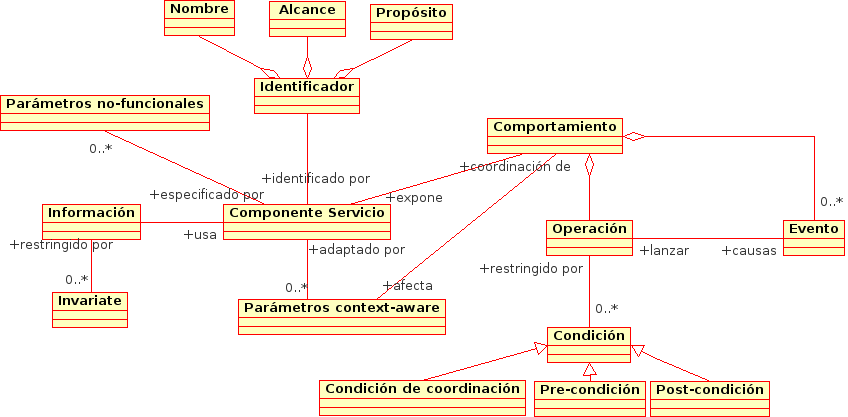
\includegraphics[width=5in,totalheight=2in]{contratoca.png}
                \caption{\small \sl Meta-modelo del contrato context-aware} \label{contratoca}
\end{center}
\end{figure}
 

Para una mejor comprensión de las componentes del modelo explicitaremos a continuación su caracterización y funciones particulares: 

\textit{Identificador} – Una componente servicio es identificada para un determinado contexto por un único nombre en el espacio de nombre.

\textit{Comportamiento} -  De acuerdo con los roles asignados en un determinado contexto, una componente servicio expone comportamientos correspondientes a provisión y pedido de operaciones, y/o publicaciones y recepción  desde/hacia cada contexto. Las operaciones pueden ser definidas en dos tipos – operaciones que ejecutan cómputos o transformaciones (tipo “update”) y operaciones que proveen algún tipo de información sobre consultas  (tipo “query”). Estas, se encuentran enteramente especificadas en base a  un contrato, con el uso de pre-condición, post-condición y condicionales para lograr la coordinación entre contratos. En las condiciones de coordinación se especifican cómo requerir y proveer operaciones, así como también los eventos publicados  y recibidos son coordinados en los momentos adecuados. Para lograr una comunicación precisa con una componente servicio, no sólo se tiene en cuenta qué operación fue provista o requerida y cómo el ejecutor ha lanzado el evento apropiado, sino también, cómo todas esas actividades están mutuamente relacionadas para ser aprovechadas por el objeto consumidor. Un evento del contexto que lanza una operación dada, puede ser parte de un conjunto de pre-condición, mientras que un evento emitido a través de una exitosa operación puede ser parte de una pos-condición. 
Las operaciones provistas y requeridas por la componente de servicio deben estar asociadas, a fin de determinar las operaciones que deben ser completadas antes de la activación de un servicio (qué es posible de ejecutarse en paralelo o ser sincronizado por otro camino). Por ejemplo, en el caso de una componente de servicio ManegadorOrden, la operación HacerOrden no puede ser invocada hasta que el servicio que la consume no esté correctamente autorizado por el componente de servicio AdministradorRegistros, o la operación deleteOrder no puede ser invocada si la operación HacerOrden con el mismo parámetro OrdenID no fue previamente completada.

\textit{Tipos de Información} –  Una componente de servicio debe  manejar, usar,  crear o tener cierta información de recursos con el propósito de proveer servicios adecuadamente.  Este elemento del contrato define el tipo de información relevante para las componentes  asociadas al contrato, así como también restricciones y reglas sobre instancias de esos tipos. Esto representa un modelo de información lógica de una componente de servicio. Formalmente, esta información de tipos puede ser considerada como definiciones de tipos de  los parámetros de las operaciones o tipos relacionados a ellos.

\textit{Configuración de Parámetros Context-Aware} – Una componente servicio depende del contexto de su actual entorno. La misma, para utilizarse en diferentes contextos logrando la adaptación a eventuales cambios debe tener definido un conjunto de parámetros de configuración.  Ejemplos de estos parámetros pueden ser: Contexto-del-Usuario (CU) - en un sentido similar a lo definido en el capítulo anterior, locación en tiempo y espacio de los servicios consumidos y suministrados. Estos parámetros, pueden ser enviados dentro de las invocaciones de las operaciones de los servicios o por medio de otros caminos, mediante componentes de servicios que pueden adaptar su comportamiento ante el cambio de contexto en una determinada situación.  
La configuración de parámetros está directamente asociada a las relaciones de las operaciones de los servicios para lograr una mejor adaptación a la medida de las circunstancias brindada por la información relevada del contexto. El concepto de la configuración de los parámetros context-aware, es un paso muy importante hacia la concepción de servicios automatizados y auto adaptables (tomando el sentido paradigmático de los teóricos de la Inteligencia Artificial).

\textit{Parámetros no funcionales} – Una componente servicio puede definir un conjunto de  los llamados parámetros no funcionales que caracterizan a la “calidad” de sus prestaciones dentro de un determinado contexto. Estos parámetros, son elementos para los consumidores de los servicios que permiten optar por el uso de un determinado  servicio, o buscar otro con el mismo o similar contrato. Como ejemplo de parámetros no funcionales podemos mencionar: Performance, Fiabilidad, Tolerancia a Fallos, Costos, Prioridad y Seguridad.


\section{DOCUMENTACIÓN DE LOS PROCESOS E-LEARNING} \label{documentacion}

Las transacciones e-learning en un AWe-lrn están definidas como secuencias de actividades asociadas con un flujo de ejecución que permite al usuario desempeñar una determinada tarea  y/o alcanzar una meta a través de la Aplicación. Entonces, un porceso de educación (o proceso e-learning - Pe-lrn) puede ser interpretada como una especificación del concepto de "workflow" en una aplicación e-learning Web, con las condiciones (restricciones) que implica la concreción de un Pe-lrn. En una transacción e-learning Web, una  $Actividad$ está  conformada por un conjunto de operaciones simples o complejas sobre datos y contenidos de la Aplicación. Como ejemplo de transacciones e-learnign se pueden mensionar un proceso en el cual un usuario (alumno) participa en un espacio de edición colaborativa (este caso será analizado posteriormente como caso de uso en las secciones posteriores) 

Entonces, las transacciones en un AWe-lrn son el camino para la representación de los Pe-lrn y proveer a los usuarios de servicios, accediendo a ellos por medio de las herramientas que los contienen (wiki, foro, video conferencia, taller, blog, etc.) La ejecución de transacciones de un AWe-lrn supone tanto la navegación a través de las herramientas, por medios de los links de las componentes hipermediles, como  el uso de sus servicios. Un ejemplo de servicio puede ser en una video conferencia la posibilidad de que un docente edite en una pizarra compartida (con sus alumnos y colaboradores) una determinada ponencia. 

El diseño de las transacciones abarcar varios niveles de abstracción, distintos formalismos pueden ser usados para su representación y documentación. Al menos tres nivels de abstracción pueden ser representados: (1) nivel conceptual, (2) nivel lógico, y (3) nivel de implementación.  El diseño conceptual permite una representación del sistema (las transacciones y su alcances) tal cual son persividas por el usuario y despejando las cuestiones de implementación. El diseño de la implementación se encuentra focalizado a proveer a los diseñadores de los AWe-lrn con todas las especificaciones necesarias para la configuración y realización de sus componenetes. El diseño lógico es un nivel intermedio del diseño de abstracción. utilizado para  trasladar las especificaciones centrales del usuario desde el diseño conceptual en terminos de  especificaciones más cercana a las implementaciones.

Al igual que lo que ocurre con todos lo artefactos de software, el diseño de una Transacción e-learning para un AWe-lrn  se puede tornar muy complejo. Cuanto más complejo sea el diseño, las confusiones entre los diseñadores (expertos en educación y analistas) y los implementadores (programadores y  encargados de la Aplicación) crecerán. Para comunicar efectivamente la idea del diseñador es necesario una apropiada documentación. Si bien la documentación textual ha sido muy utilizada para describir detalles de implementaciones de bajo nivel, teniendo en cuenta que el diseño de las transacciones e-learning se describen en un  nivel conceptual, es más adecuado una representación gráfica. 

Existen diferentes aportes  directamente relacionado a modelos "visuales" en forma de documentación gráfica \cite{5,10,12}. En este contexto los modelos visuales son representaciones de sistemas de software que soportan multiples perspectivas. Para el caso del diseño de las transacciones e-learning, una vista puede ser representada por una series de diagramas pertenecientes a UML (Unified Modeling Language) \cite{UML} 

Los antecedentes relevantes que se relacionan con lo que entendemos por diseño de Pe-lrn, fueron estudiados de los aportes del campo del métodos de diseños para aplicaciones Web experimentados en los últimos años. Concretamente se pueden mensionar ADM (Atzeni y Parente, 2001), OO-H (Koch et al., 2003), OOHDM (Schmid and Rossi, 2004) y UWAT+ (Distante, 2005).

UWAT+ es un meta-modelo para la descripción de los distintos aspectos de Transacciones Web de manera holística. Es una extensión del Modelo de Diseño de Transacciones que forma  parte del framework UWA (Ubiquitous Web Applications) \cite{UWA}. Inspirado en este modelo y extendiendolo para la contensión de los contratos, se describe una adaptación para el diseño de transacciónes e-learning en un AWe-lrn.

\section {UWATc+: una adaptación de UWAT+ para el modelado de proceso e-learning} \label{uwatc}

Si bien los métodos de diseño de Transacciones de UWAT+ pueden ser utilizados para la representación de transacciones e-learning, es necesario efecutuar adecuaciones que tengan en cuenta la inclusión a los contratos (según sección \ref{contrato}). Tal cual fue mensionado en la sección \ref{intro}, desde la perspectiva de los diseñadores, los contratos deben ser visto como una pieza de software para la instrumentación de los servicios de las herramientas. En consecuencia, es necesario tener un modelo que permita una mejor representación de los contratos, la visualización de su inserción en los servicios y las relaciones que en ellos se representan (relaciones entre objetos que implementan servicios, usuarios y herramientas en la Aplicación). 


La figura \ref{drobab} se muestra un diagrama de clase UML que representa a los conceptos, las relaciones entre conceptos y los modelos para la representación de transacciones. Los esquemas en color blanco pertenecen al modelo original UWAT+. El rectángulo y los esquemas grices describen los objetos, modelos y relaciones que  que conforman el nuevo modelo denominado UWATc+.

	\begin{figure}[!h]
        \begin{center}
	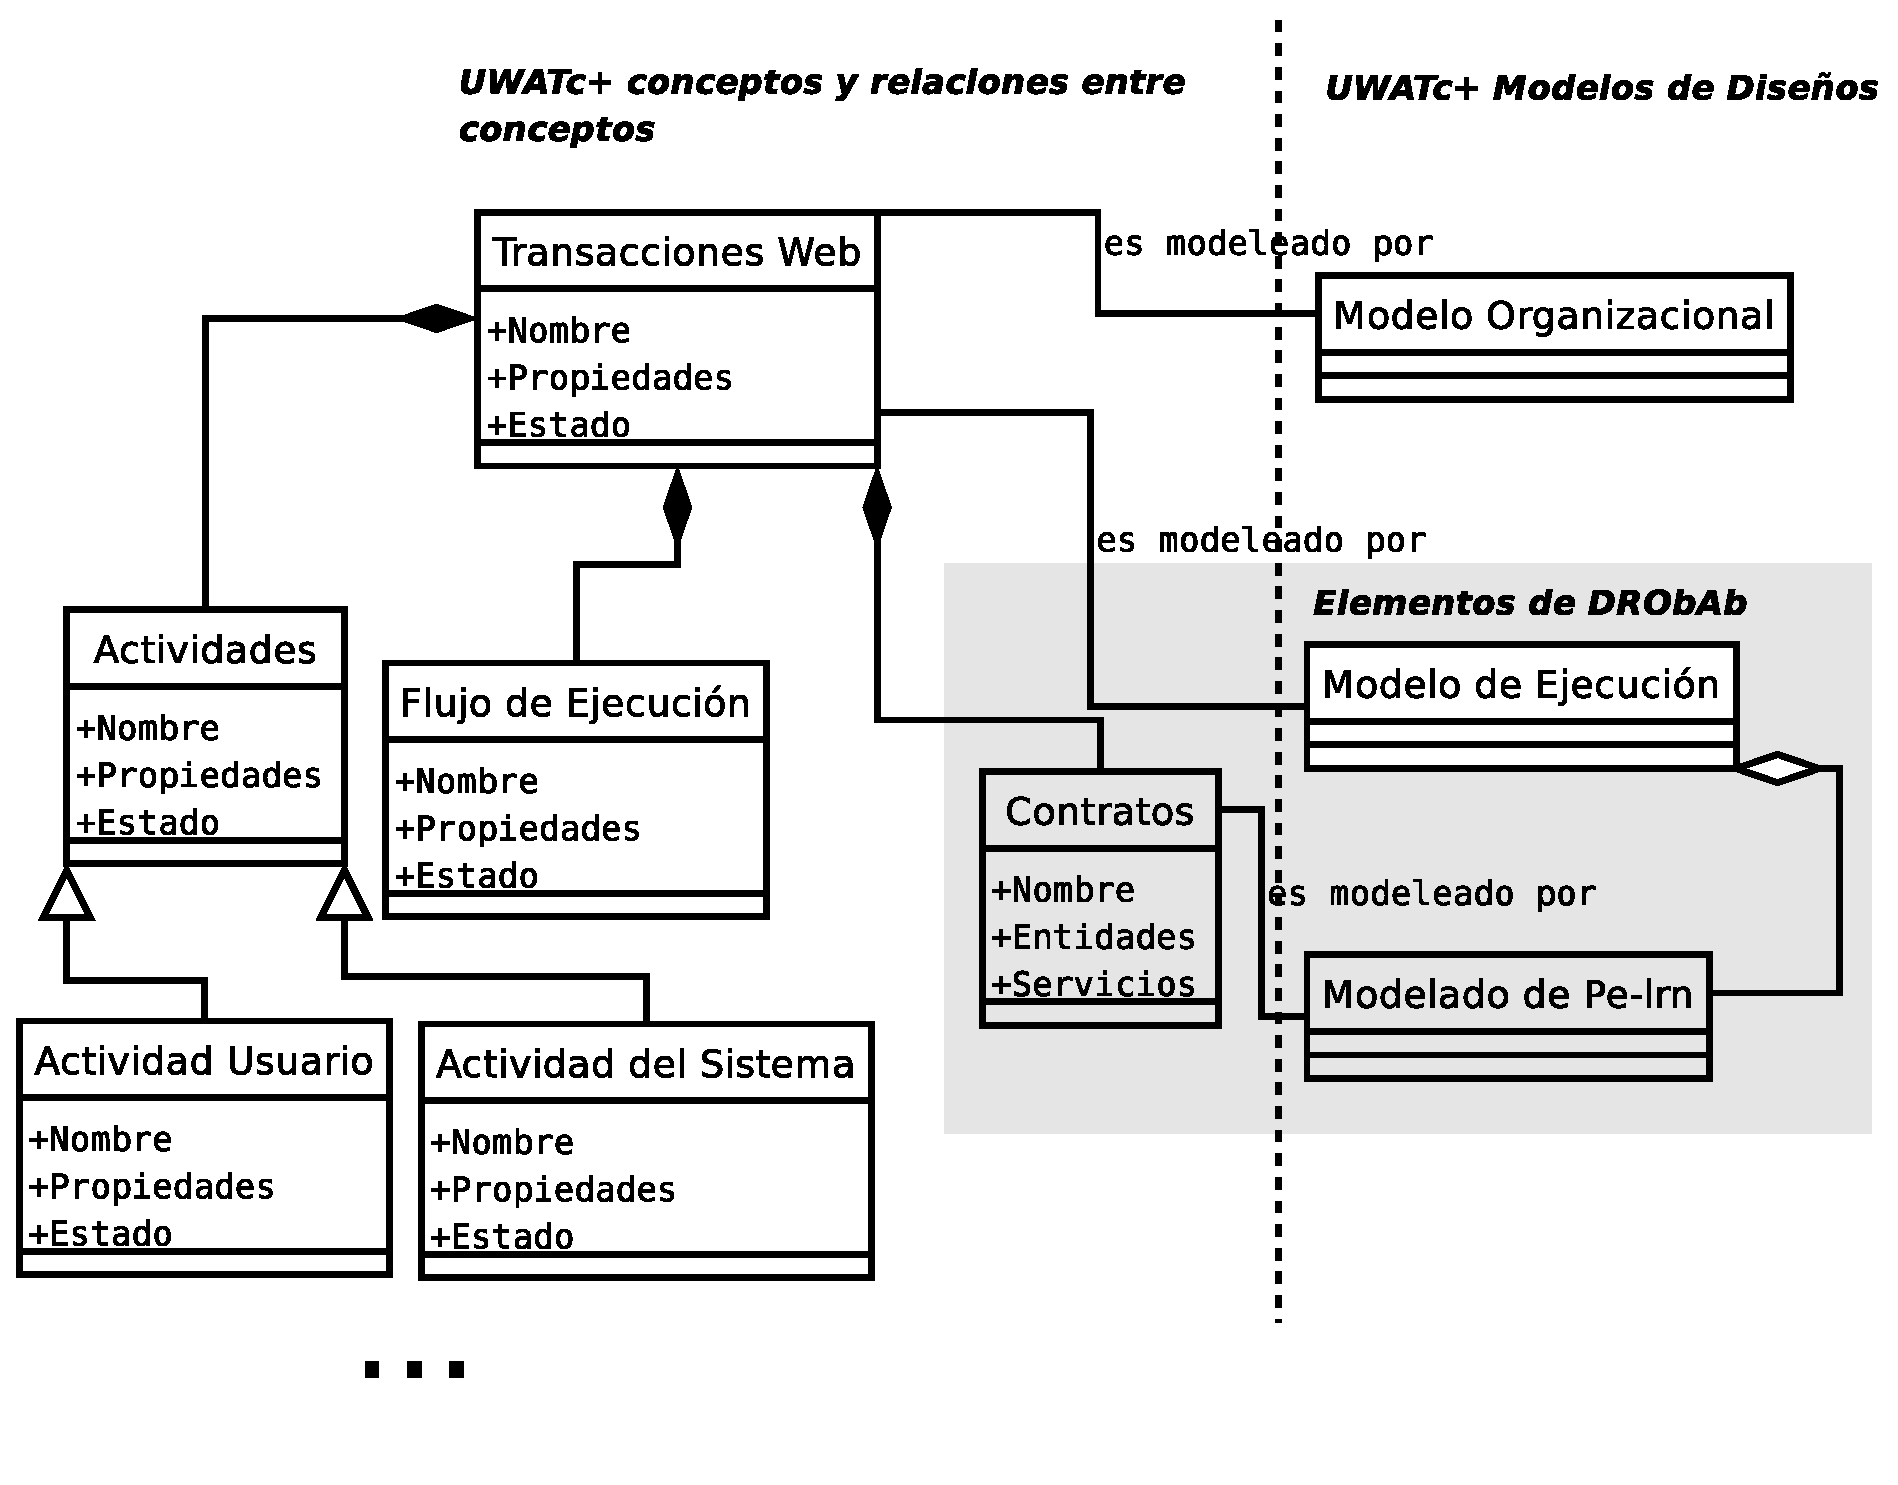
\includegraphics[width=5 in,totalheight=3 in]{drobab.eps}
	\caption{\small \sl UWATc+ modelo conceptual y de diseño} \label{drobab}
         \end{center}
         \end{figure}


Como se describe en el diagrama, una Transacción Web es un objeto complejo (conceptual) compuestos por dos tipos de objetos principales pertenecientes al modelo original de UWAT+ y un tercer objeto  agregado para la representación de los contratos pertenecientes a las Transacciones e-learning. En el primer grupo se encuentra $Actividad$ para la distinción de las actividades de los usuarios y del sistema. El objeto $Flujo de Ejecución$ representa del órden lógico y temporal para la ejecución de las actividades comprendidas en las Transacciones. A su vez, una Transacción Web puede ser descripta por el $Modelo Organizacional$ (desde el punto de vista estático) y el $Modelo de Ejecución$ para la definición de las reglas de ejecución de la componente actividad (desde el punto de vista dinámico). 

Cuando una Transacción Web contiene un contrato (definida como transacción e-learning) debe ser incluida una nueva componente para el diseño (representrada en la figura como una relación de agregación en el $Modelo de Ejecución$), conjuntamente con un nuevo modelo de diseño, $Modelo de Pe-lrn$, que permitira la representación del contrato (caracterizada como relación de asoción con el objeto $Contrato$).

De esta manera quedan conformados los elementos que componen el modelo UWATc+ (rectángulo gris) y sus relaciones con el modelo original UWAT+. A continuación se describe en detalle el modelo usado por UWATc+ para el diseño de los transacciones que utilizan contratos (transacciones e-learning). 


\subsection{Requerimientos para el diseño de trasacciones e-learning}

En esta sección se describen la caracterización de dos tipos representativo de requerimiento que motivaron la creación de este nuevo modelo de diseño de los Pe-lrn (definidos en la sección \ref{intro}). En base a experiencias recogidas por el grupo del proyecto Obra Abierta en el diseño y configuración de Aplicaciones e-learning, se presentarán dos tipos de requerimientos que deben ser cubiertos por el modelo de diseño. En primer lugar se enuncian cuestiones técnicas de diseño (desde el punto de vista de la Ingeniría de Software), seguido de un comentario sobre el tipo de Transacciones que el diseñador puede especificar a través del diseño.

\begin{itemize}

\item Especificar como son afectadas la ejecución de las actividades por los objetos contratos. 
\\

La relación de una actividad con un contrato se produce cuando existen objetos interrelacionados por medio de un contrato \cite{fiadeiro}. De esta manera, el diseñador debe porder documentar las información de los objetos involucrados, sus métodos y parámetros. El contrato representa un tipo diferente de relación a la origianal entre los objetos, con la propiedad de re-configurado en tiempo de ejecución. Característica que permiten una mejor adaptación a los requerimientos que resuelven las transacciones e-learning.

\item  Definir cual y como la  información de los objetos contratos ("information object" \cite{informationobject}) es afectada por la ejecución de las Actividades.
\\

Una actividad funcional conciste en la ejecución de uno a más operaciones elementales (inserción, borrado, modificación, etc.) sobre los datos de la Aplicación y la información de los objetos contratos envuelta en la actividad. El modelo de diseño de Transacciones e-learning debe permitir al diseñador definir cuales operaciones del contrato son fundamentales para cada actitividad, modelando el camino en que cada actividad elemental afecta la información de los objetos involucrados (modificando sus instancias por medios de sus ejecuciones).
\end{itemize}


\section {DISEÑO DE PROCESOS E-LEARNING CON UWATC+} \label{diseno}

En esta sección se describen los resultados de la apliación de UWATc+ para el espacio dedicado al libro "Hacia un dispositivo hipermedial contex-aware Dinámico. Educación e investigación para el campo audiovisual interactivo" (San Martín P, et. al) \cite{libro}.  Este  modelo fue aplicado parcialmente para el diseño de los requerimientos fundamentales y el modelado del compertamiento funcional enmarcado bajo la perspectiva de proyecto Obra Abierta - mensionado anteriormente. Se presentará un caso de uso para ejemplificar el diseño de un Pe-lrn en la Aplicación e-learning para Obra Abierta. El diseño describe parte del proceso en que un usuario hace uso de los servicios de edición de la herramienta Foro a tráves de un contrato. 

	\begin{figure}[!h]
        \begin{center}
	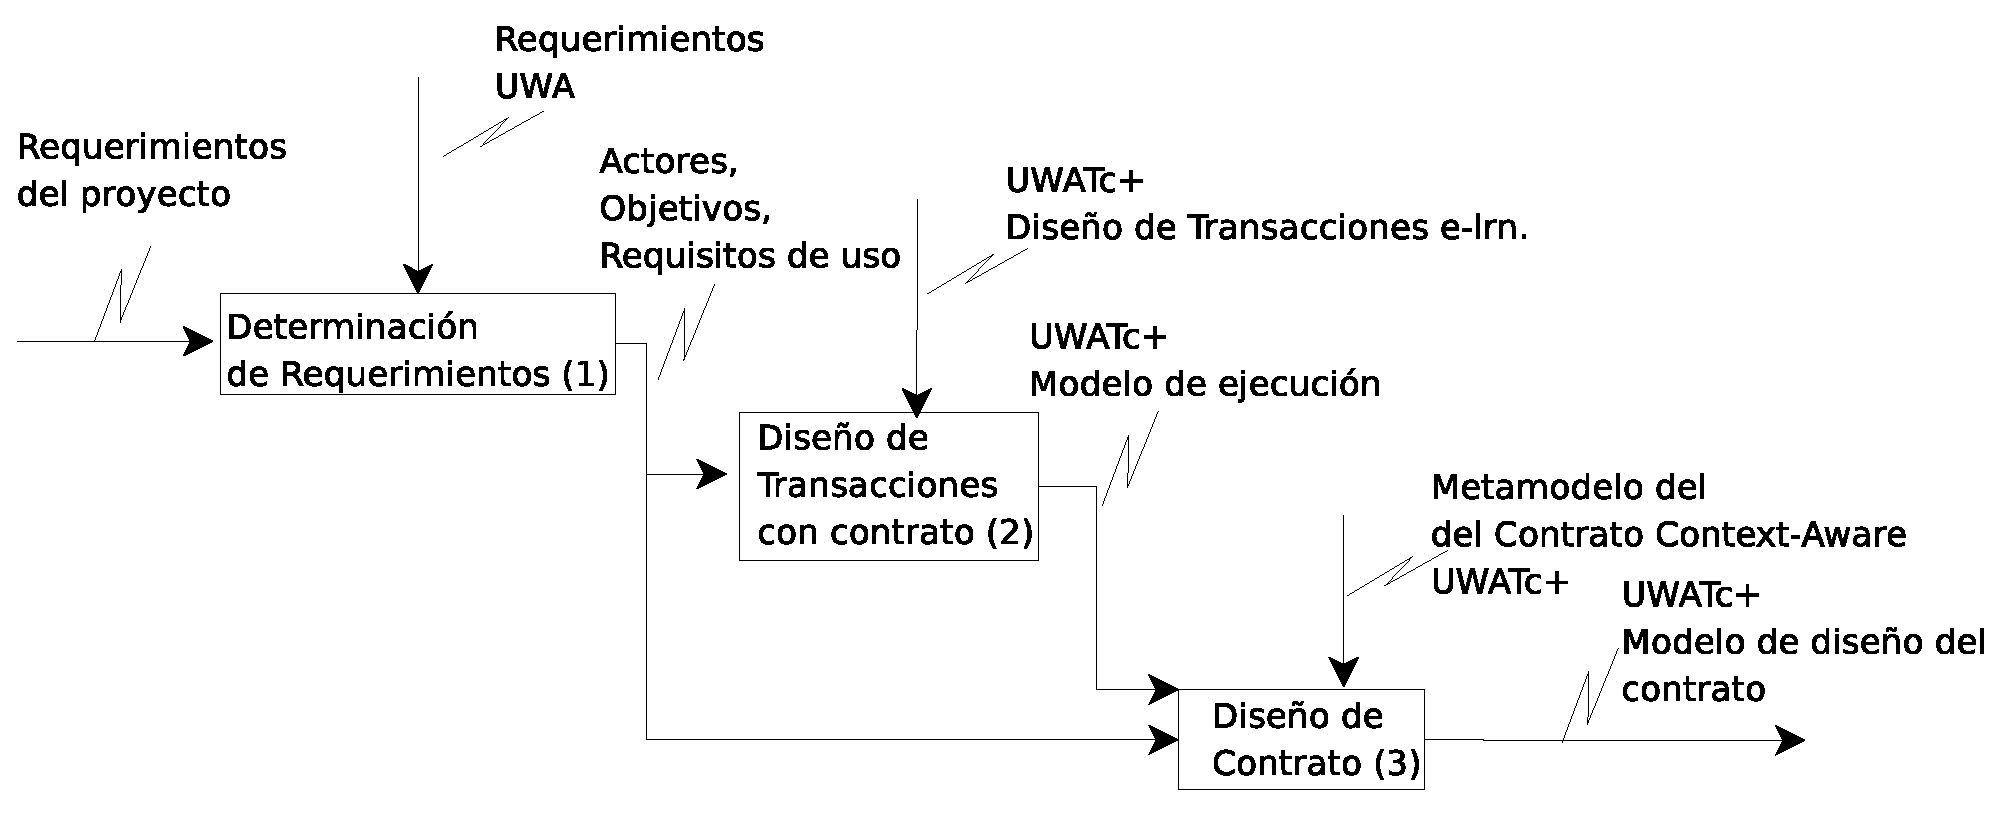
\includegraphics[width=6 in,totalheight=2 in]{procesodisenoNuevo.eps}
	\caption{\small \sl El proceso de diseñar Pe-lrn en un AWe-lrn con UWATc+} \label{procesodediseno}
         \end{center}
         \end{figure}



El diagrama de la figura \ref{procesodediseno} muestra una adaptación del diseño de procesos de UWA \cite{UWA} que se utiliza en UWATc+ para el diseño de transacciones con contratos. Para ilustrar el proceso de diseño se utiliza la notación IDEF0 (IDEF-0, 1993). En comparación con la metodología original de UWAT+, se agregaron las fases del diseño de contrato y fue modificado el modelo de diseño de la transacciones. Además, fueron exluidas las fases de "diseño de la información" y "diseño de publicación". Las fases del procesos de diseño son: (1) Determinación de Requerimientos; (2) Diseño de transacciones con contrato; (3) Diseño de contrato.

\subsection{Determinación de Requerimientos} \label{sdr}

La fase de Determinación de Requerimientos toma como entrada las especificaciones del proyecto y produce, por medio de un mecanismo de refinamiento, las siguientes salidas: Cada actor con su objetivos relativo. Los requerimientos para la contrucción y configuración de un AWe-lrn.
 
El modelo utilizado es orientado a objetivos: cada actor se identifica con al menos un objetivo, i.e, una abstracción de los objetivos que a través de la aplicación se debe alcanzar; cada objetivo es refinado en otros sub-ojetivos, hasta poder definir el requerimiento en un bajo nivel suficiente para poder ser implementado. Este fase es similar a la descripta en (UWA Consortium, 2001) \cite{UWA}. 

	\begin{figure}[!h]
        	\begin{center}
		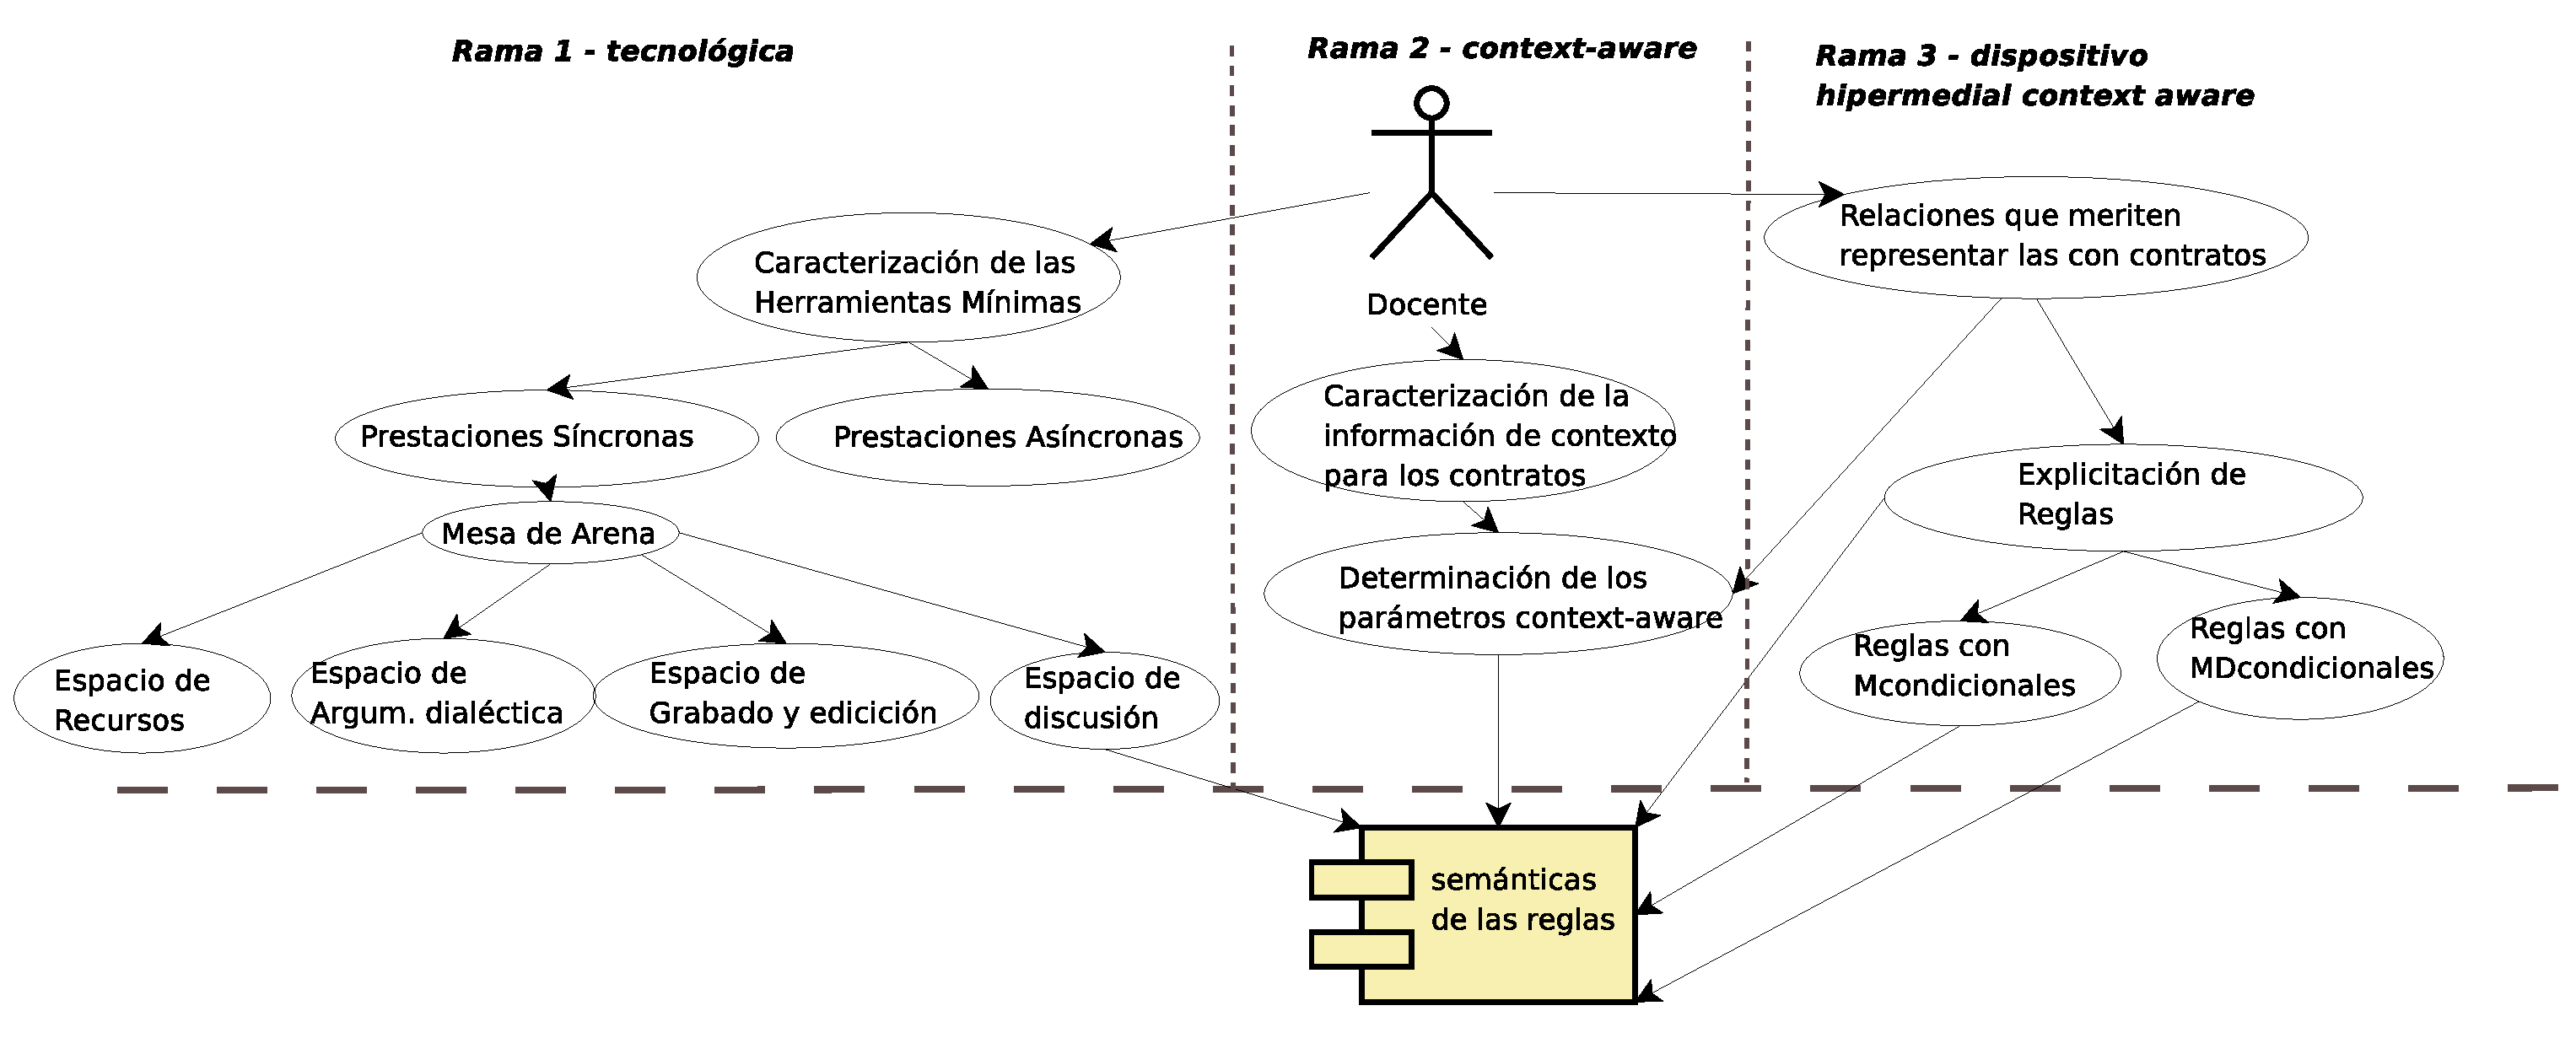
\includegraphics[width= 5 in,totalheight=3 in]{Requerimientos.eps}
                \caption{\small \sl Objetivos de al alto nivel  para el PdEAI} \label{requerimientos}
         	\end{center}
         \end{figure}

Para este caso de uso, atendiendo a los lineamientos en \cite{libro}, se describe parte del modelo original donde se carateriza los objetivos involucrado con un actor relevante del sistema. A su vez, a medida que se van derivando los sub-objetivos comienzan a establecerse requerimientos concernientes a la teoría de coordinación de contratos context-aware \cite{libro5,fiadeiro}. En la figura \ref{requerimientos} dicha situación ocurre en la derivación de las tres ramas de objetivos y sub-objetivos, influyendo directamente en la composición de la componente contrato. En este caso, tomando desde la \textit{\textbf{rama 1}} un servicio de una herramienta de un espacio de discusión (herramienta Foro); de la \textit{\textbf{rama 2}} se desprenden las información necesaria para poder articular dicho servicio teniendo en cuenta la información de contexto;  la \textit{\textbf{rama 3}} aporta el consenso de los expertos (del dominio e-learning) para la inclusión de los contratos en aquellas relaciones que mantendrán las propiedades de la Aplicación e-learning con la inclusión de los contratos \cite{libro5}. A través de este modelo, se logra un primer acercameinto sobre como se relaciona un contrato con: los requerimientos, el tipo de objetivos para cada requerimiento y los actores del sistema. 

\subsection{Diseño de Transacciones e-learning}

El diseño de transacciones e-learning retoma la misma idea y modelo propuesto por UWAT+ para el diseño de transacciones \cite{UWAT}. Partiendo de los resultados de la fase de \textit{Determinación de Requerimientos}, fundamentalmente de la caracterización de los contratos, pueden ser seleccionados una series de transacciones, i.e., objetivos que requieran la ejecución de una o más Actividades para su cumplido. Para cada uno de los objetivos que incluya contrato deben ser diseñadas transacciones e-learning (de igual forma que con las transacciones en UWAT+), los cuales en principio deben ser establecidos desde un punto de vista estático (en este trabajo no abordaremos tal consideración) y luego, desde un punto de vista dinámico por medio de un modelo de ejecución. En la figura \ref{modelodeejecucion} se muestra una porción del modelo de ejecución de un transacción e-learning cuyo contrato asociado fue caracterizado en la fase de \textit{Determinación de Requerimientos} (figura \ref{requerimientos}, sección \ref{sdr}). En el diseño se describe el flujo de ejecución entre las Actividades de la transacción. El modelo de ejecución es una adaptación del diagrama de actividades de UML \cite{7} en el que las Actividades y sub-Actividades están representadas por estados (óvalos), y el flujo de ejecución entre ellos se representa por medio de transiciones (arcos). Los óvalos con el símbolo (*) - un asterisco etre paréntesis - a una Actividad que representa a un conjunto de actividades compuestas, y cuyo modelo de ejecución debe ser representado con otro diagrama. Un óvalo simple representa una Activiad Elemental. Un óvalo color griz indica una Actividad compuesta de las sub-actividad que se encuentra dentro. Una sub-Actividad representada con un óvalo color griz indica que es dependiente de la Actividad que la contiene, esto quiere decir que su ejecución estará acopañada por otra sub-Actividad y no puede ser incluida en otra composición. Los arcos de lineas continuas indican flujos de ejecución oblicagorio (transacciones hacia Actividades requeridas), mientras que los actos con lineas de puntos representan flujo de ejecuciones opcionales  (transacciones hacia Actividades opcionales).
 
Cada relación posible entre actividades es representada por medio de una arco entre ellas. A cada arco se le asocia un texto que indica bajo que condiciones se produce la transacción, o el resultado de la ejecución de la Actividad de origen. Para describir como colaboran los usuarios de la aplicación en la ejecución de la Actitivades puede ser anexado un diagrama UML Swimlanes. 

Cuando una Actividad ejecuta servicios implementados por contratos, entonces, se establece un arco saliente hacia un contrato. El contrato tiene un nombre y entre paréntices se indican cuales son los objetos participantes (en el caso de tener ese tipo de información). Para represetarlo visualmente se utiliza el estereotipo del elemento componente de UML. Las Actividades que influyan en la modificación de los contratos en tiempo de ejecución se conectan a través de un arco de linea de puntos, igual a los utilizado en la representación de los flujos opcionales. Los detalles implementativos del contratos se detallan en un diagrama aperte, perteneciente a la fase descripta en la siguiente sección.

	\begin{figure}[!h]
        \begin{center}

	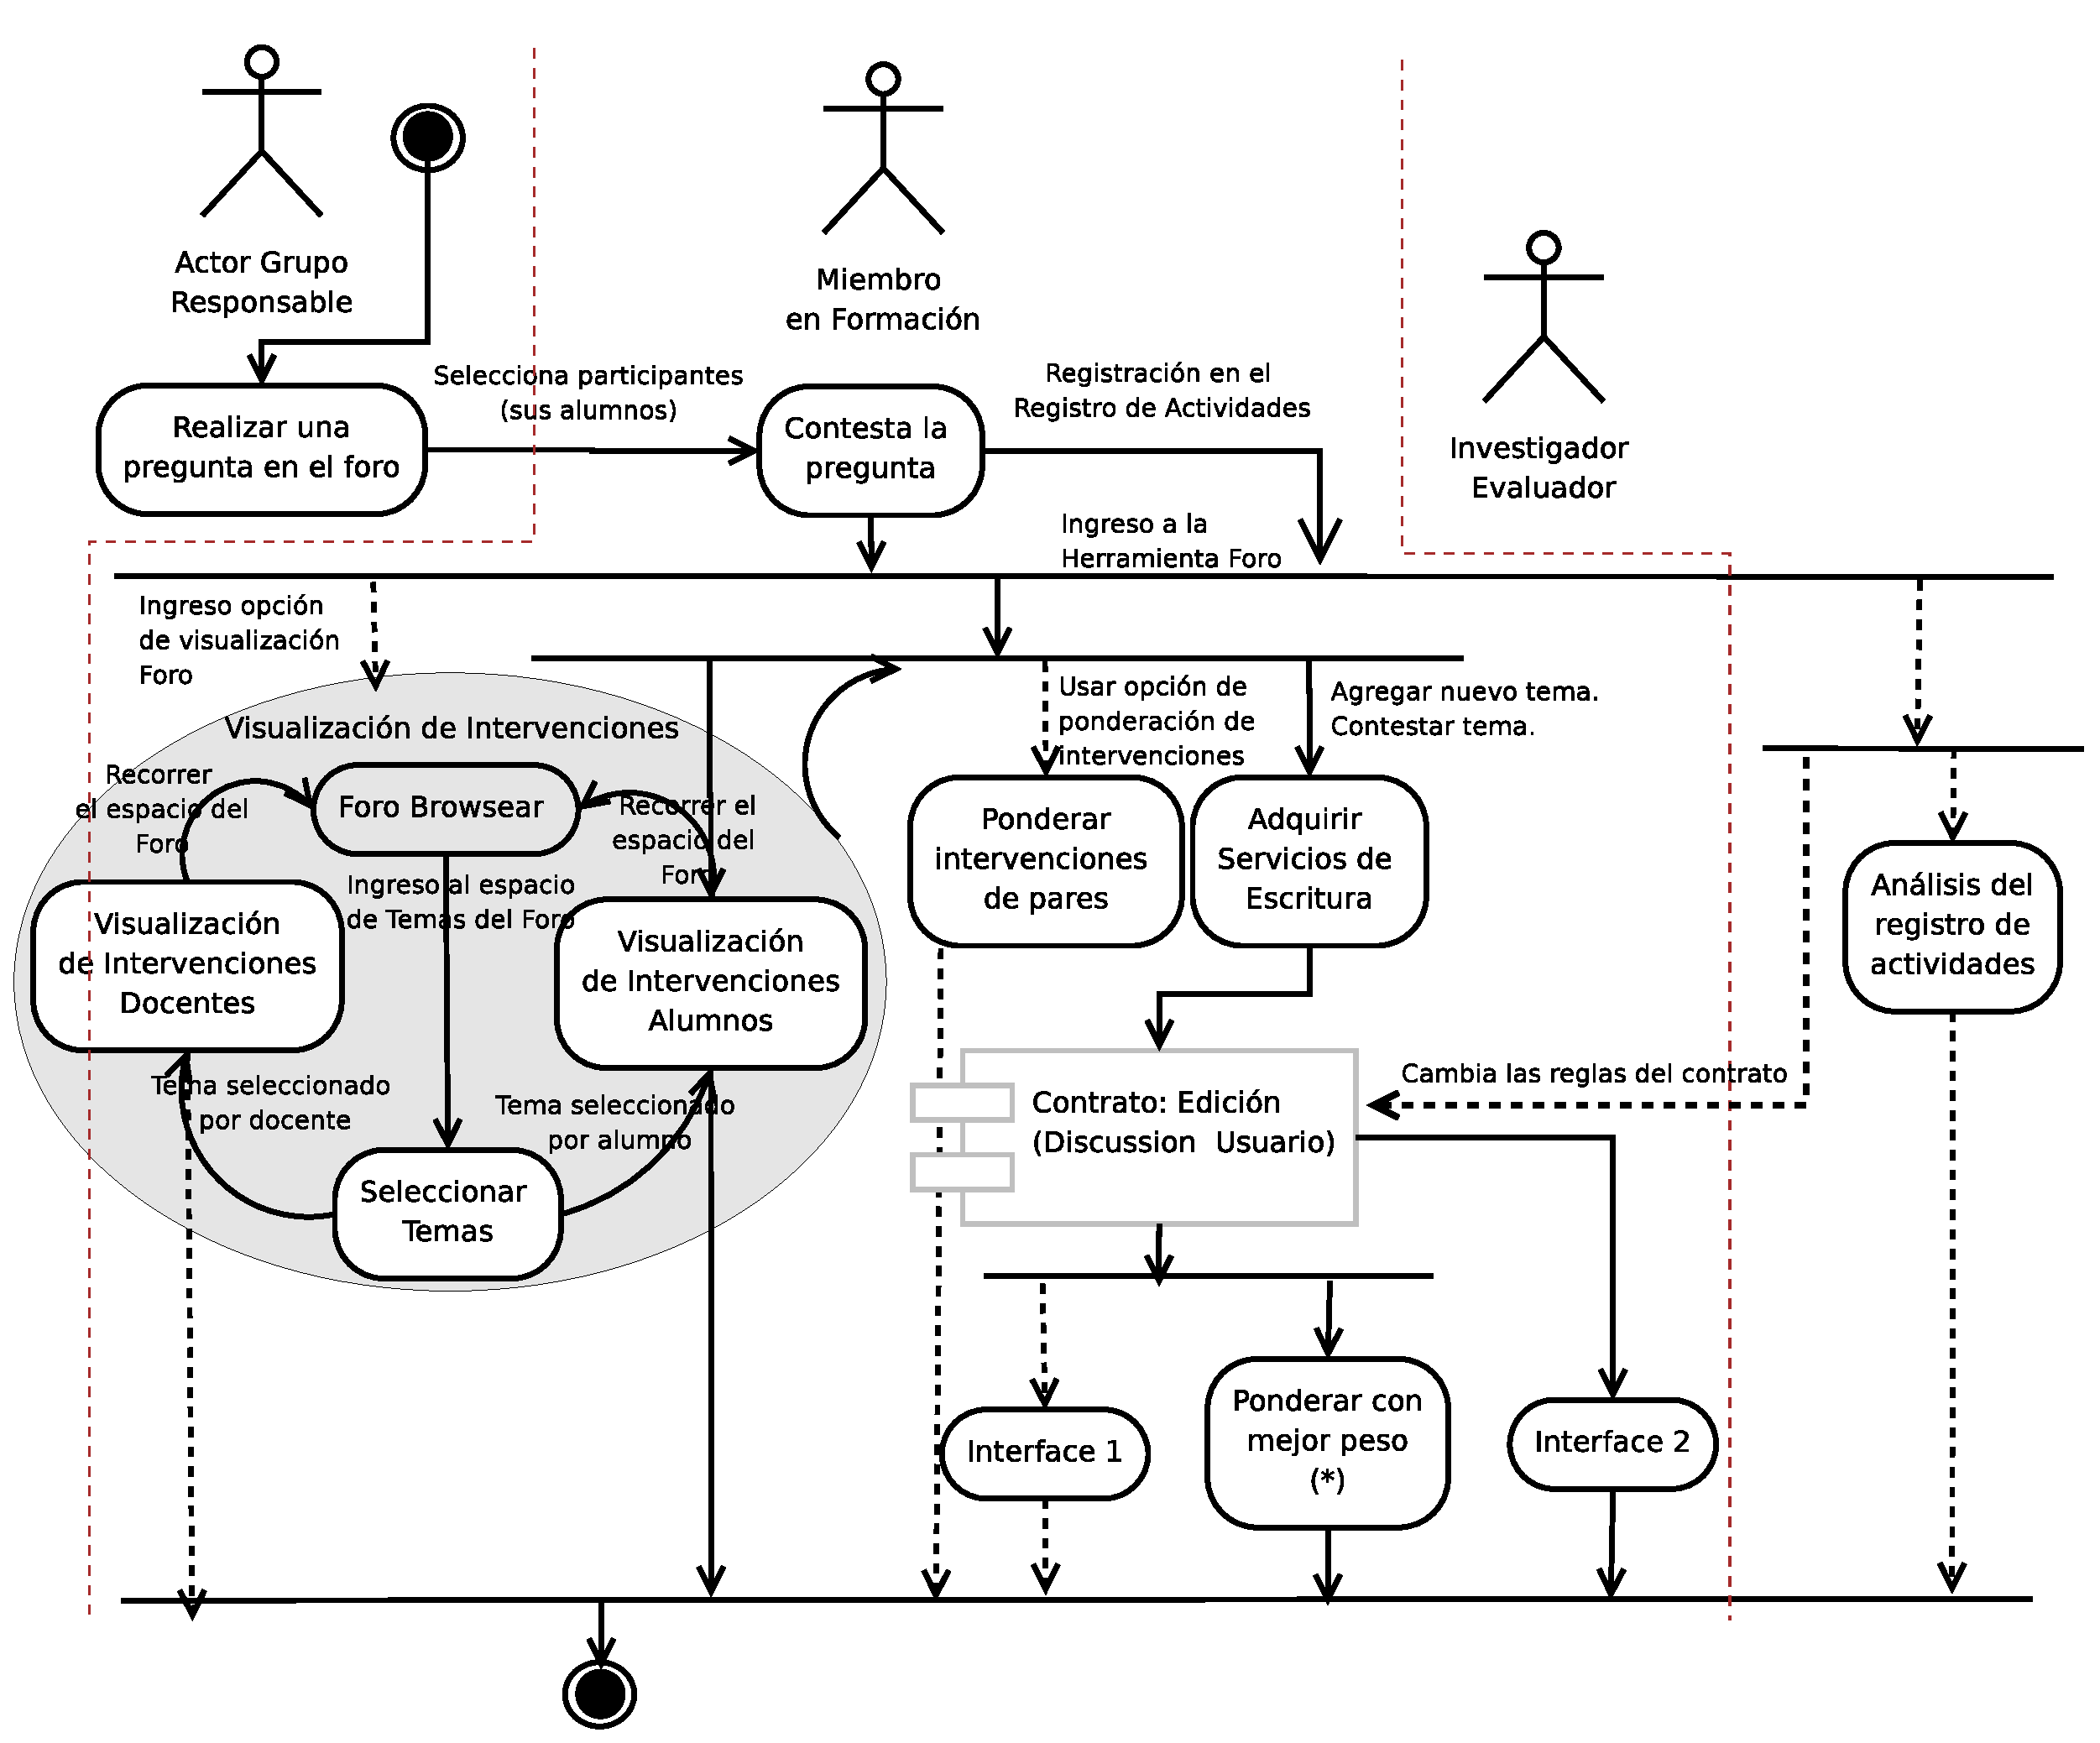
\includegraphics[width=5 in,totalheight=4 in]{proceso.eps}
                                    \caption{\small \sl Modelo de ejecución de Procesos de Educación e investigación} \label{modelodeejecucion}
         \end{center}
         \end{figure}


Por ejemplo, una de las opciones de la herramienta Foro de Obra Abierta (http://200.80.157.171:8080/portal) es la visualización de las intervensiones de los usuarios en el Foro. Un usuario docente puede seleccionar la opción "Foro" de la página principal de la Aplicación, luego seleccionar el tipo de "vista" (mediante un "comboBox") para ingresar en modo "browser" donde se muestran las intervenciones de los usuarios por temas. Una vez seleccionado el tema (por medio de la Actividad "Seleccionar Tema", figura \ref{modelodeejecucion}), es posible ingresar al espacio de las intervenciones de los usuarios por medio de los roles de docente o alumno. Los docentes y alumnos tienen diferentes tipos de ·"vistas", permisos y servicios asociados (representadas en las actividades: "Visuazación de Intervensiones Docentes" y "Visualización de Intervensiones Alumnos"). A  través del Browser (Actividad "Foro Browser") se recorre todo el contendido del espacio y al mismo tiempo puede ser seleccionado otro tema para visualizar.

En cambio, si la opción seleccionado es añadir o responder temas, se ingresa a unas páginas Web configuradas para editar texto (por medio de la Actividad "Adquirir servicios de escritura"). Algunos de los servivios de edición y configuración de opciones son implementadas a través del contrato "Edición" (representado por la figura de la componente UML, con el contorno color griz). El flujo de ejecución, luego de la intervención de los contrato, dependerán de las reglas de coordinación y se representan con los arcos salientes similares a los usados para representar las relaciones entre estados.


\subsection{Diagrama de un Contrato}

Existen diferentes formas de representación de los contratos definidos en la sección \ref{contrato}, la herramienta  CED (Coordination Development Environment) \footnote{CED: es el primer prototipo de una herramienta que implementa el uso de la coordinación de contrato en aplicaciones Java. La herramienta pertenece a ATX Sofware (www.atxsoftware.com.ar);fue desarrolada en Java y es de código abierta.} los implementa a través de un lenguaje llamado Oblog \cite{lenguajeoblog}. En \cite{communit} se muestra como a través de CommUnity se definen primitivas de modelado y técnicas de diseño basadas en la separación de la "coordinación" del "cómputo". 

En UWATc+ se brinda un diagrama de representación de contrato, donde se describen todos los datos que lo instancian. Cada tipo de dato y valor, pertenece a un elemento del meta-modelo de la figura \ref{contratoca}. Teniendo en cuenta la figura \ref{diagramacontrato}, en primer lugar (item 1) se identifican los objetos participantes en el contrato; en el ejemplo de la figura \ref{diagramacontrato} $DiscussionAction$ y $UserAction$ hacen referencias a dos clases reales pertenecente a la implementación de la herramienta Foro y Usuarios de la herramientra Abra Abierta, respectivamente. Luego, se identifican los nombres de los parámetros context-aware significativos para el contrato, alineados en la misma columna del objeto que lo comparte (item 2). En Servicios (item 3) deben ser represetados los métodos del objeto, que al ser ejecutados, probocan la intervención del contrato. Para este ejemplo $initState$ y $getIdentifier$  son ejecutados cuando un usuario ingresa a la herramienta Foro de y las posteriores funcionalidades (servicios) disponibles  dependen de la ejecución del contrato $Edición$ (la figura \ref{modelodeejecucion} muestra la superposición del contrato entre los servicios de edición y las nuevas interfaces o funcionalidades). Los siguentes filas (items 4 y 5) se refieren a las pre y post-condiciones que se deben cumplir en la ejecución del contrato. Por último se explicitan las reglas de coordinación. Siguiendo con el ejemplo, en la parte del condicional $u.contexto=’l1;p1;docente;r1;c1;’$ verifica si el contexto del usuario $u$ está compuesto por la locación $l1$, tienen el perfil $p1$, es un $docente$, cumple el rol $r1$ y pertenece a la categoría $c1$ (este tipo de representación de contexto se encuentra desarrollado en \cite{libro}). En cuanto a la acción de la regla de coordinación, continuando con el mismo ejemplo, se induce la ejecución del método $showMessage$ del objeto $d$ (DiscussionAction). El final del diagrama está dedicado a comentarios generales; cada comentario dede ir acompañado con el número de item (1,2,3,4,5 o 6) al que hace referencia. 

\begin{center}

\small{ 

\begin{tabular}{|l|p{20mm}|p{55mm}|p{1mm}|p{55mm}|} 
		\hline 
\multicolumn{5}{|c|}{\textbf{Contrato:} Edición}\\
		
\hline 
1.& \textit{Participantes}: 	& \textbf{d}:DiscussionAction && \textbf{u}:UserAction \\
\hline 
2.& \textit{Param. c-a}: 	&	state, portlet, rundata, context &&  	context$_$identifier, identifier 	\\
3.& \textit{Servicios}:		& 	initState()		 	 &&	getIdentifier()				\\
4.& \textit{Pre-Cond}: 		& existe $<contexto>$ 			&& existe $<contexto>$  \\
5.& \textit{Pos-Cond}: 		& modifica $<contexto>$ 		&& \\
\hline 
6.& \textit{Reglas      de Coordinación}: & \multicolumn{3}{l|}{{\textbf{Si} \textbf{u}.contexto='p1;d;r1;c1;' \textbf{entonces} \textbf{d}.showMessage(data,string)}}  \\
\hline 

\multicolumn{5}{|c|}{\textbf{Comentario}} \\
\multicolumn{5}{|l|}{1. DiscussionAction y  UserAction  pertenecen a clases implementadas en JAVA del proyecto Sakai. } \\
\multicolumn{5}{|l|}{4 y 5. $<contexto>$ refiere a un objeto donde se oculta toda la información de contexto} \\ 

\multicolumn{5}{|l|} {que caracterisa a los usuarios de la plataforma} \\



\hline
\end{tabular} 
}
\end{center}

    \begin{figure}
	\begin{center}
	\caption{\small \sl Diagrama del contrato: Edición} \label{diagramacontrato}
         \end{center}
  \end{figure}


\section {CONCLUSIÓN}

En base a la experiencia recogida en el proyecto Obra Abierta, es posible asegurar que la implemntación del modelo de diseño UWATc en el ciclo de vida del desarrollo Aplicaciones E-Learning permitió un mejor entendimientos entre los expertos en educación, diseñadores y programadores. El modelo también ayudó en la compresión de la teoría de coordinación de contrato aplicada a transacciones para Aplicaciones e-learning.


%-------------------------  bibliografía ----------------------------------


\begin{thebibliography}{1}

\bibitem{libro5} Sartorio A., San Martin P., 2007. {Sistemas Context-Aware en dispositivos hipermediales dinámicos para educación e investigación}. \textit{Universidad Nacional de Quilmes (UNQ). Capítulo. En impresión.}

\bibitem{libro} San Martín P., Sartorio A., Guarnieri G., De la Riestra M., 2007. {Hacia un dispositivo hipermedial context aware dinámico. Educación e Investigación para el campo audiovisual interactivo}. \textit{Universidad Nacional de Quilmes (UNQ). Libro. En impresión.}


\bibitem {5} Hartmann, J.; Huang, S.; and Tilley, S. {Documenting
Software Systems with Views II: An Integrated Approach
Based on XML.} Proceedings of the 19th Annual
International Conference on Systems Documentation
(SIGDOC 2001: October 21-24, 2001; Santa Fe, NM), pp.
237-246. ACM Press: New York, NY, 2001.

\bibitem {10} Tilley, S. and Huang, S. {Documenting Software Systems
with Views III: Towards a Task-Oriented Classification of
Program Visualization Techniques.} Proceedings of the 20th
Annual International Conference on Systems Documentation
(SIGDOC 2002: October 20-23, 2002; Toronto, Canada), pp.
226-233. ACM Press: New York, NY, 2002.

\bibitem {12} Tilley, S.; Müller, H.; and Orgun, M. {Documenting
Software Systems with Views.} \textit{Proceedings of the 10th
Annual International Conference on Systems Documentation
(SIGDOC ‘92: October 13-16, 1992; Ottawa, Canada), pp.
211-219. ACM Press: New York, NY, 1992.}

\bibitem {UWA} UWA Consortium (2002). {Ubiquitous web applications.} \textit{Proceedings of The eBusiness and eWork Conference (e2002), 16–18 October, Prague, Czech Republic.}

\bibitem {UWAT} Distante, D., Tilley, S. and Huang, S. (2004b). {Documenting software systems with views IV:
documenting web transaction design with UWAT+.} P\textit{roceedings of the 22nd International
Conference on Design of Communication (SIGDOC 2004), Memphis, TN, New York, NY:
ACM Press, 10–13 October.}


\bibitem {transaccion web}

Brambilla, M., Ceri, S., Fraternali, P. and Manolescu, I. (2006).{ Process modeling in web
applications.} \textit{ACM Transactions on Software Engineering and Methodology (TOSEM), in print.}


\bibitem {fiadeiro}

L.F.Andrade and J.L.Fiadeiro. {Interconnecting Objects via Contracts.}  I\textit{n UML'99 – Beyond the Standard,
R.France and B.Rumpe (eds), LNCS 1723, Springer Verlag 1999, 566-583.}


\bibitem {lenguajeoblog}

The Oblog Corporation. {The Oblog Specification Language.}  http:// www.oblog.com/tech/spec.html


\bibitem {7} Object Management Group (OMG). {Unified Language
Modeling Specification (Version 2.0).} \textit{Online at
www.omg.org, 2004.}


\bibitem {UML}

Murphy  S., Tilley S. and Huang S. {The 4th Workshop on
Graphical Documentation: UML Style Guidelines.} \textit{To be
held as part of The 22nd Annual International Conference on
Design of Communication (SIGDOC 2004: October 10-13,
2004; Memphis, TN)}

\bibitem {informationobject}

Distante, D., Tilley, S. and Huang, S. (2004b). {Documenting software systems with views IV:
documenting web transaction design with UWAT+.} \textit{Proceedings of the 22nd International
Conference on Design of Communication (SIGDOC 2004), Memphis, TN, New York, NY:
ACM, 10–13 October.}


\bibitem {communit}

D.Gelernter and N.Carriero. {Coordination Languages and
their Significance}.\textit{ Communications ACM 35, 2, pp. 97-
107, 1992.}

\end{thebibliography}

\end{document}
